\documentclass[conference,harvard,brazil,english]{sbatex}
\usepackage[utf8]{inputenc}
\usepackage{float}
\usepackage{ae}
\usepackage{amsfonts, amssymb}
\usepackage{amsmath}
\usepackage{graphicx}
\usepackage{indentfirst}
\usepackage{ae}
\usepackage{gensymb}
\usepackage{caption} 
\usepackage{epstopdf}
\usepackage{leading}

\makeatletter
\def\verbatim@font{\normalfont\ttfamily\footnotesize}
\makeatother
\usepackage{amsmath}
% --------------------------------------------------
\begin{document}

    \title{Projeto, Construção, Modelagem e Controle de um Pendulo Invertido Dinâmico}
    \author{Thalles Oliveira Campagnani}{thallescampagnani@gmail.com}
    \twocolumn[
        \maketitle
        \selectlanguage{brazil}
        \begin{abstract}
            O presente trabalho apresenta o projeto e construção de uma planta de controle no formato de uma motocicleta, e por isso a mesma é modelada como um pendulo invertido, e possui as mesmas dinâmicas que uma bicicleta. É apresentado a modelagem da planta, as linearizações do modelo, projeto de controladores proporcionais e derivativos pelo método do lugar geométrico das raízes, e por fim, comparativos das as respostas de cada sistema, entre a planta física e simulada.
        \end{abstract}
        \keywords{Pendulo Invertido Dinâmico, Dinâmicas de Bicicleta, Linearização de Modelos, Lugar Geométrico das Raízes, Controlador Proporcional.}
        \selectlanguage{english}
        \begin{abstract}
            The present work presents the design and construction of a control plant in the shape of a motorcycle, so it is modeled as an inverted pendulum, and has the same dynamics as a bicycle. It is presented the modeling of the plant, linearizations of the model, design of proportional controllers and derivatives by the root locus method, and finally, comparative of the responses of each system, between the physical and simulated plant.
        \end{abstract}
        \keywords{Dynamic Inverted Pendulum, Bicycle Dynamics, Linearization of Models, Geometric Place of Roots, Proportional Controller.}
    ]
    
    \selectlanguage{brazil}
    
    \section{Introdução}
        
        O presente artigo irá apresentar um projeto mecânico, elétrico, eletrônico, eletromecânico e computacional de uma planta de controle, a modelagem e projetos de controladores para a mesma.
        
        A planta consiste basicamente em um veiculo de duas rodas com atuador cada. Uma desta manterá fixo o ângulo que seu eixo faz com o corpo da planta, sendo ela responsável por atuar na velocidade tangencial através de um motor acoplado a mesma. A outra irá variar o ângulo que seu eixo faz com o corpo da planta através de um servo motor, sendo ela responsável pelo raio de curvatura que a planta fará em torno de um centro instantâneo de rotação.
        
        A combinação de velocidade tangencial e raio de curvatura são responsáveis por gerar momento no corpo da mesma, alterando o ângulo que o corpo da planta faz em relação a gravidade. Este ângulo é a variável de saída da planta e é a variável a ser controlada, a partir de uma velocidade tangencial constante e variando o ângulo da roda dianteira.
    
    \section{Objetivos}
    
        Os objetivos gerais são: projetar e construir uma planta de controle, modela-la, valida-lo (o modelo), realizar estudos em malha aberta para prever o comportamento em malha fechada, projetar um controlador que estabilize a planta, e por ultimo realizar estudos em malha fechada.
        
        Os objetivos específicos referente a planta são: Projetar e construir a planta de controle como uma miniatura de motocicleta, robusta mecanicamente para suportar eventuais quedas em movimentos e colisões frontais. Devera ter pneus capazes de absorver impactos e vibrações, e rugosos o suficiente para o atrito não permitir derrapagem nas curvas. A roda traseira deverá ter um grau de liberdade angular apenas em relação ao corpo da planta, enquanto a dianteira deverá ter dois graus de liberdade angulares na mesma relação. A planta deverá ser naturalmente instável, com dois atuadores, um para atuar na velocidade tangencial e outro para atuar no raio de curvatura através da variação do ângulo do eixo . Um sensor deverá ser capaz de medir a inclinação da mesma em relação a gravidade, um microcontrolador irá processar as informações do sensor e emitir um sinal de controle para os atuadores e emitir sinal via WI-FI para um dispositivo remoto capitar dados em tempo real e alterar parâmetros do controlador. Por fim a planta deverá possuir bateria com autonomia suficiente para se realizar os testes.
        
        Apesar da planta possuir dois atuadores, apenas um, o servo motor, será a entrada de sinal para a planta. O outro atuador, o motor cc, atuará em malha aberta a um valor constante. E para efeitos de calculo, será considerado que a saída do atuador (velocidade tangencial) será constante.
        
        Os objetivos específicos referente a ao controlador são: Depois de modelada e obtido a função de transferência da planta, utilizar o método do lugar geométrico das raízes para projetar um controlador proporcional de ganho K. Caso o controlador proporcional não torne a planta assintoticamente estável, projetar outro controlador através de outro método com o fim de estabilizar a mesma.
        
    \section{Projeto da Planta}
    
        \subsection{Projeto Mecânico}
            
            O projeto da parte mecânica da planta foi feito com o auxilio de \textit{software} de \textit{CAD} (Desenho Técnico Assistido por Computador). Parte das peças foram projetadas para serem impressas em impressoras 3D, enquanto outras passam por processos de usinagem, como por exemplo elementos de maquinas como rolamentos.
            
            A maior peça, comumentemente chamada de "quadro", é o corpo da planta e tem função estrutural. Uma outra peça, batizada comumentemente de "garfo", tem a função de alterar o ângulo que o eixo da roda dianteira faz com o corpo da planta, além de funções estruturais. Ambas peças foram projetadas para serem impressas em material \textit{ABS}. O acoplamento entre o "garfo" o corpo da planta foi projetado para ser intermediado por um conjunto de rolamentos radiais e axiais, a fim de restringir os graus de liberdade do acoplamento para apenas um angular, conferir resistência mecânica, baixo atrito e possibilitar ainda transmissão de movimento de um atuador, servo motor, sem transferir esforços mecânicos para tal. Foi projetado ainda no corpo da planta um "para-choques" dianteiro para absorver impactos e proteger a roda dianteira em eventuais colisões.
            
            As duas rodas foram projetadas para serem torneadas a partir de um tarugo de nylon, a traseira se diferindo da dianteira apenas por um canal que serve de polia, para através de uma correia, possibilitar a transmissão de movimento entre a mesma um atuador eletromecânico, motor de corrente continua, afixado no corpo da planta logo acima da roda traseira. O nylon foi escolhido pela fácil usinabilidade, baixa densidade, e resistência mecânica suficiente para o projeto. O acoplamento entre roda traseira e o corpo da planta, e entre a roda dianteira e o "garfo", foram ambos projetados para funcionar através de rolamentos radiais, a fim de proporcionar um grau de liberdade angular apenas para os mesmos, e baixo atrito.
            
            Os pneus revestem a roda e foram projetados para serem confeccionados a partir da extrusão de silicone (acima do seu ponto de fusão) deixando o núcleo oco e parte externa maciça, para depois serem torneadas as partes externas dando o formato final. O silicone foi escolhido para os pneus pela sua maleabilidade, onde, deixando seu núcleo oco, pretende-se absorver vibrações provenientes do formato da superfície do solo e conformar a superfície do pneu aumentando a área de contato com o solo.
            
            Os elementos de maquinas utilizados nos acoplamentos foram escolhidos de acordo com o preço e tamanho já que estes serão submetidos a esforços muito menores do que são capazes de suportar.
            
        \subsection{Projeto Elétrico, Eletrônico e Eletromecânico}
        
            Os componentes elétricos, eletrônicos e eletromecânicos serão todos reciclados de outros projetos ou equipamentos fora de funcionamento.
            
            Componentes eletrônicos: o conversor de sinais será um microcontrolador, os sensores serão acelerômetros e giroscópios, e o responsável pela distribuição da tensão da bateria ao restante dos componentes uma Ponte-H com regulador de tensão. 
            
            O microcontrolador escolhido foi o "Wemos D1 Mini" devido o mesmo ter Wi-Fi integrado.
            O sensores escolhidos estão embutidos em uma placa chamada "MPU-6050". Ela possui 3 sensores acelerômetros e 3 sensores giroscópios perpendiculares entre si, e ainda um "processador de movimentos digital", \textit{DMP}, que coleta, processa e filtra os dados dos 6 sensores a fim calcular a direção da gravidade em tempo real.
            A ponte-H escolhida foi um placa que contem o chip "Ln-298" e um circuito regular de tensão. Este chip alimentará o motor cc e ele suporta a corrente drenada pelo mesmo. O regulador de tensão alimentará o microcontrolador e os sensores.
            
            Componentes eletromecânicos: dois atuadores, o primeiro um motor de corrente continua e o segundo um servo motor. 
            
            O motor-cc foi reciclado a partir de uma impressora de papel e atende o requisito de tirar a motocicleta da inercia. 
            O servo motor foi escolhido o "MGTOWER Mg955" disponível de outro projeto já que este possui velocidade angular em vazio parecida com a maioria dos servos no mercado de baixo custo.
            
            Componentes elétricos: duas baterias de lítio de 3.7V e cabos elétricos.
            
            As baterias serão ligadas em serie totalizando 7,4V para alimentar o servo motor e a placa da ponte h com regular de tensão.
        
        \subsection{Projeto Computacional}
        
            Inicialmente foi estabelecido os protocolos de comunicação: Para o envio de sinal ao servo motor foi escolhido "modulação por largura de pulso", \textit{PWM}, para receber informações do \textit{DMP} do sensor "MPU-6050" foi escolhido \textit{I2C} e por ultimo para comunicação com dispositivos remotos via Wi-Fi foi escolhido TCP-IP e via USB foi escolhido comunicação Serial. Para intermediar o controle dos periféricos responsáveis por cada protocolo foram utilizadas bibliotecas \textit{open-source's} compatíveis.
            
            Foi desenvolvida uma função para atuar no servo motor com base nos dados do sensor seguindo o molde de controlador proporcional e derivativo. A respeito dos ganhos do controlador eles são inicialmente $0$ para ambos.
            
            Foi desenvolvida uma outra função que permite alterar os parâmetros (ganhos) do controlador através de informações recebidas via USB e/ou Wi-Fi. A mesma função faz envio dos dados do sensor em tempo real via mesmos meios.
            
    \section{Construção da Planta}
    
        O quadro e o garfo foram impressos em Plástico ABS através de Impressora 3D, e acoplados um no outro utilizando rolamentos axiais e radiais conforme projetado.
        
        As rodas foram concebidas usinando-as em tornos mecânicos e os pneus foram feitos preenchendo o canal das mesmas com silicone - de uma certa forma que o interior não ficasse $100\%$ preenchido isto afim de absorver impactos e vibrações. Depois conjunto pneu-roda foi usinado a fim de dar acabamento áspero a superfície do pneu e o formato de circunferência ao mesmo. Por fim foram acopladas ao garfo e ao quadro utilizando rolamentos radiais.
        
        O motor foi afixado, e a imagem a baixo é o resultado destas etapas concluídas:
        
        \begin{figure}[h]
            \centering
            %\hspace{-18mm}
            \includegraphics[width=4cm]{imagens/planta/motinhaTL.jpg}
            \caption{Vista da Planta em Construção}
        \end{figure}
        
        Foi impresso e afixado a parte superior do quadro o suporte do atuador, servo motor, e acrescentado uma adaptação de um $arm$  ao conjunto de acoplamento do garfo ao atuador, conforme imagem abaixo:
        
        \begin{figure}[h]
            \centering
            %\hspace{-18mm}
            \includegraphics[width=4cm]{imagens/planta/arm.jpg}
            \caption{Acoplamento do Servo Motor}
        \end{figure}
        
        O motor foi acoplado o motor a roda através do sistema de polia e correia, conforme visto na imagem abaixo:
        
        \begin{figure}[h]
            \centering
            %\hspace{-18mm}
            \includegraphics[width=4cm]{imagens/planta/PoliaMotinha.jpg}
            \caption{Acoplamento do Motor CC}
        \end{figure}
        
        Foi incrementado uma barra roscada no quadro ao final da execução do projeto para proteger a planta em eventuais quedas que ocasionalmente poderão ocorrer no funcionamento da mesma, e também para possibilitar um ajuste fino na posição do centro de gravidade.
        
        Por fim, foram afixados ao quadro então o motor, ponte h, microcontrolador, baterias e e o sensor. Depois instalados os cabos elétricos e compilado o algorítimo para serem iniciados os testes, que no fim se demonstraram satisfatórios. O resultado final pode ser visto na primeira figura 4.
        
    \section{Modelagem da Planta}
        
        A planta é modelada como um pendulo invertido. O que a difere das demais é a cinemática envolvida no ângulo de atuação, ou seja, o ângulo de esterço da roda dianteira, e dinâmica da planta, que não leva em conta massa da mesma.
        
         Antes de modelar a equação diferencial que rege a planta, é necessário fazer esquematizações, considerações, e modelar a aceleração centípeda em função do ângulo de esterço da roda dianteira.
        
        \subsection{Esquematizações e Considerações}
        
            É considerado que toda a massa da planta, $m$, está concentrada em um único ponto, sendo este o Centro de Gravidade, $C_G$.
            
            \begin{figure}[h]
                \centering
                \includegraphics[width=6cm]{imagens/planta/PlantaRealCG.jpg}
                \caption{Vista Lateral da Planta}
            \end{figure}
            
            Faz-se a necessidade de criar um referencial móvel na planta, já que, esta se desloca no tempo e espaço. Este referencial terá como nome dos eixos coordenados: $X'$, $Y'$ e $Z'$, sendo estes perpendiculares entre si, $X'$ colinear com o eixo da roda traseira e $Y'$ normal ao plano que contem o eixo de ambas rodas.
            
            É  necessário saber a posição do $C_G$ no espaço. Será considerado que posição referente a dimensão $X'$ é a mesma do centro geométrico da planta. Já para as posições nas dimensões $Y'$ e $Z'$ serão consideradas posições arbitrarias medidas respectivamente pela distancia entre o $CG$ e o eixo traseiro, $d_{CG}$, e pela  distancia do $C_G$ ao ponto de contato da roda com o solo, $h$. A figura abaixo representa as esquematizações feitas por meio da vista lateral, além da distancia entre eixos, $d$.
            
            \begin{figure}[h]
                \centering
                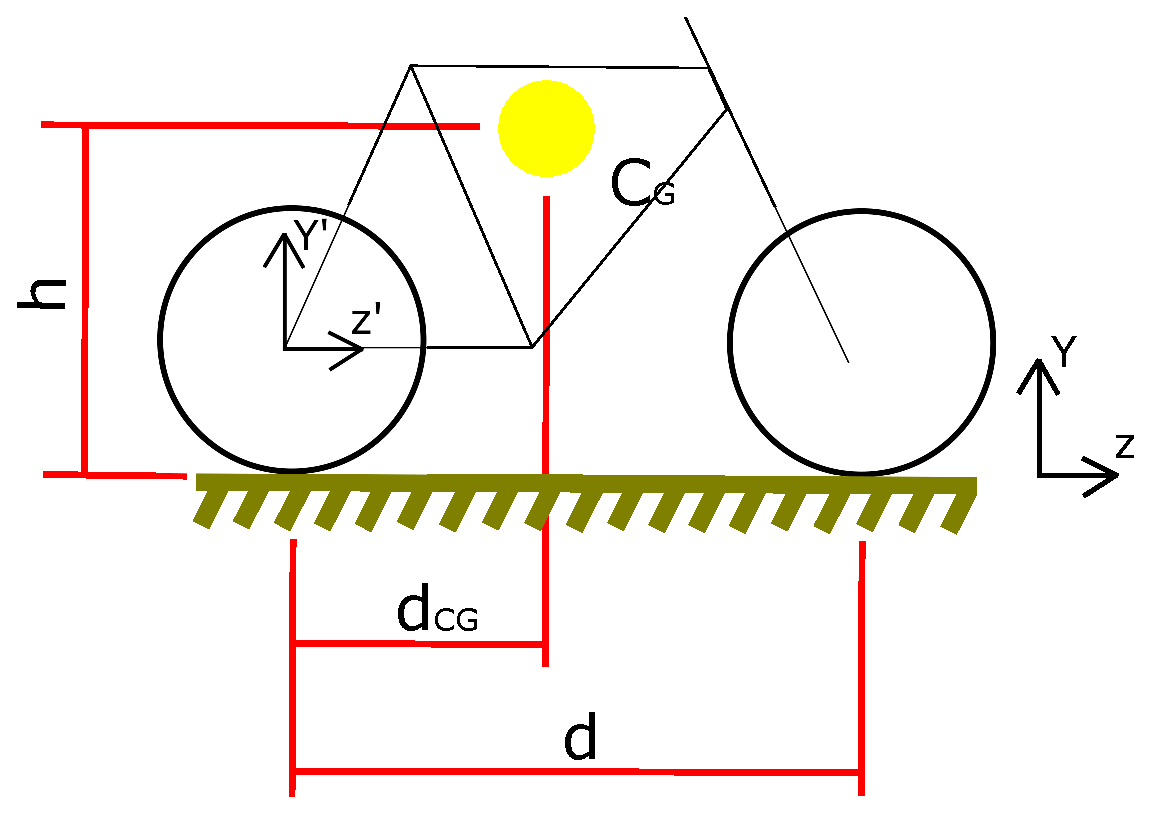
\includegraphics[width=7cm]{imagens/geometria/VistaLateral.eps}
                \caption{Vista Lateral Esquemática}
            \end{figure}
            
            O ponto de encontro dos eixos das rodas é denominado Centro de Curvatura, $C_C$, a distancia dele ao centro da roda dianteira gera o Raio de Curvatura da Roda Dianteira, $R_D$, a distancia dele ao centro roda traseira gera o Raio de Curvatura da Roda Traseira, $R_T$, e a distancia dele ao $C_G$ gera o Raio de Curvatura do Centro de Gravidade, $R_{CG}$. O ângulo formado entre $R_T$ e $R_D$ é ângulo de esterço da roda dianteira, denominado $\alpha$, e este é o ângulo de entrada da planta.  O ângulo formado entre $R_T$ e $R_{CG}$ é denominado $\beta$. Estas esquematizações podem ser vistas na figura abaixo que representa a vista superior.
            
            \begin{figure}[h]
                \centering
                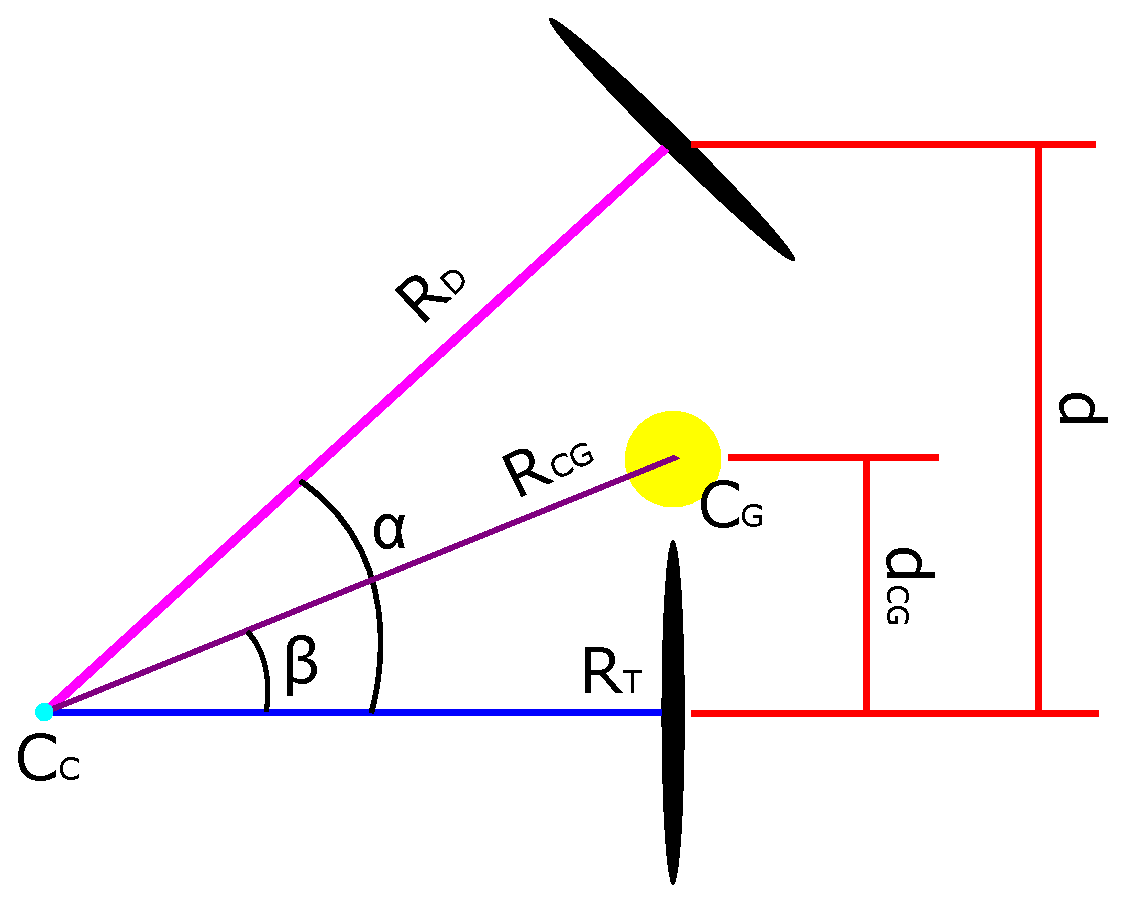
\includegraphics[width=7cm]{imagens/geometria/VistaSuperiorGeometria.eps}
                \caption{Vista Superior Esquemática - Geométrica}
            \end{figure}
            
            Será considerado que o corpo da planta não gira em torno de $X'$, que gira diretamente dependentemente do deslocamento tangencial e do valor de $\alpha$ na direção de $Y'$, ou seja, serão desconsiderado possíveis escorregamentos dos pneus, e, por fim, que a planta gira livremente na direção $Z'$, sendo sua aceleração angular diretamente dependente da resultante das acelerações lineares que o $C_G$ está sujeito.
            
            A aceleração centípeda resultante no $C_G$, simplesmente $a_c$, possui a mesma direção de $R_{CG}$. Naturalmente, somente a componente $X'$ desta aceleração gera momento em $Z'$, logo, é necessário decompô-la nesta direção, ou seja, obter $(a_c)_{X'}$ . A fim de simplificar nomenclaturas denominaremos $(a_c)_{X'}$ como somente $a_{cx}$. A figura abaixo mostra novamente a vista superior, porém com as novas informações.

            \begin{figure}[h]
            \centering
            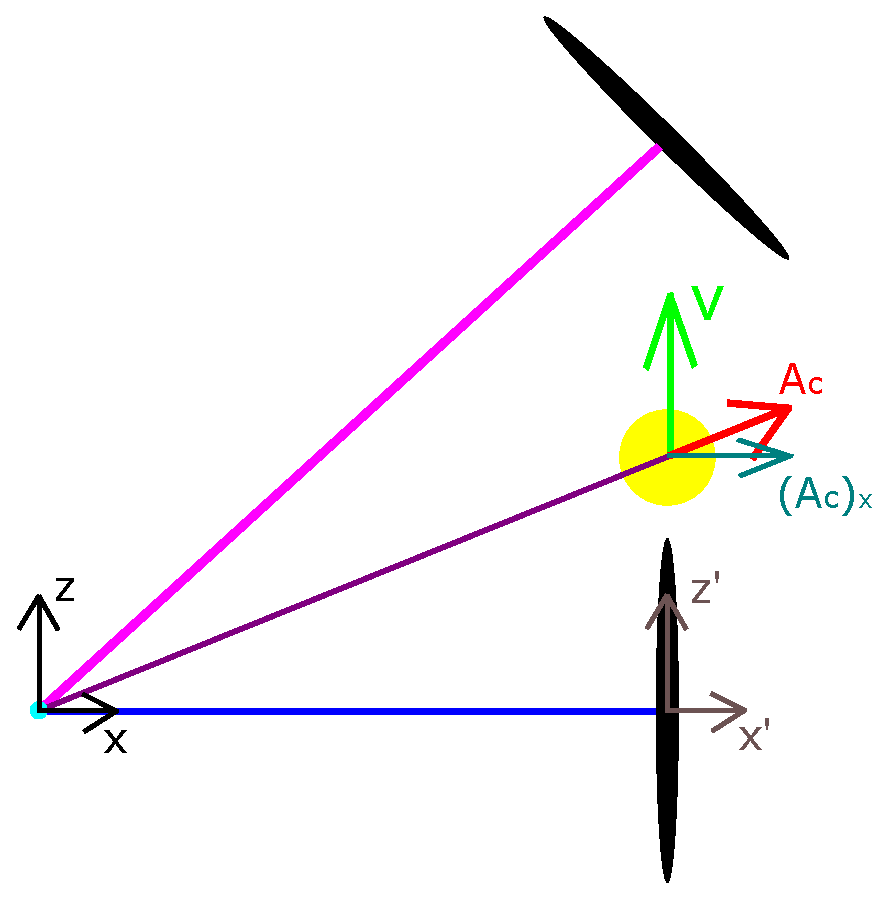
\includegraphics[width=6cm]{imagens/geometria/VistaSuperiorVetorial.eps}
            \caption{Vista Superior Esquemática - Vetorial}
            \end{figure}
            
        \subsection{Modelagem cinemática em função do ângulo de esterço}
        
            O ângulo de esterço da roda dianteira gera, partindo do pressuposto que $v!=0$, um valor de $a_{cx}$, que este será usado na modelagem da equação diferencial. Faz-se então a necessidade de encontrar essa relação, e para tal, será feita uma serie de algebrismos trigonométricos.
            
            Primeiro é encontrada a relação entre $R_t$ e $\alpha$.
            
            \begin{equation}
                \tan(\alpha) = \frac{d}{R_t} \Rightarrow R_t = \frac{d}{\tan(\alpha)}
            \end{equation}
            
            Através de $R_t$ é possível descobrir $ R_{CG}$ sabendo $d_{CG}$.
            
            \begin{eqnarray}
                R_{CG}^2 = R_t^2 + d_{CG}^2 \nonumber \\
                \Rightarrow R_{CG} = \sqrt{R_t^2 + d_{CG}^2} = \sqrt{\frac{d^2}{\tan^2(\alpha)} + d_{CG}^2}
            \end{eqnarray}
            
            É possível obter $\beta$ com através das relações já obtidas:
            
            \begin{eqnarray}
                \tan(\beta) = \frac{d_{CG}}{Rt} = \frac{d_{CG} \tan(\alpha)}{d} \nonumber \\
                \Rightarrow \beta = \arctan ( \frac{d_{CG} \tan (\alpha) }{d} )
            \end{eqnarray}
            
            A equação abaixo da a relação entre $a_c$ e $R_{CG}$ sabendo $v$. O ângulo $\beta$ pode ser usado para então encontrar $a_{cx}$
            
            \begin{equation}
                a_c= \frac{v^2}{R_{CG}} \Rightarrow a_{cx} = \frac{v^2}{R_{CG}}cos(\beta)
            \end{equation}
            
            Substituindo (2) e (3) na equação (4) temos que:
            
            \begin{equation}
                a_{cx} = \frac{v^2}{\sqrt{\frac{d^2}{\tan^2(\alpha)} + d_{CG}^2}}cos(arc\tan(\frac{d_{CG} \tan(\alpha)}{d}))
            \end{equation}
            
            É conhecido que:
            
            \begin{equation}
                cos(arc\tan (w)) = \frac{1}{\sqrt{w^2+1}}
            \end{equation}
            
            Logo,
            
            \begin{equation}
                a_{cx} (\alpha) = \frac{v^2}{\sqrt{\frac{(d^2}{\tan^2(\alpha)} + d_{CG}^2}   \sqrt{(\frac{d_{CG} \tan(\alpha)}{d})^2+1}}
            \end{equation}
            
            Portanto:
            
            \begin{equation}
                a_{cx} (\alpha) = \frac{v^2\tan(\alpha)d}{\tan^2(\alpha)d_{CG}^2+d^2}
            \end{equation}
            
            Ou ainda, caso seja necessário considerar $v$ uma variável:
            
            \begin{equation}
                a_{cx}(\alpha, v) = \frac{v^2\tan(\alpha)d}{\tan^2(\alpha)d_{CG}^2+d^2}
            \end{equation}
            
            A função $a_{cx}(\alpha)$  retorna o valor exato da componente $X'$ da aceleração centrípeta em função de $\alpha$, porém é necessário obter uma função mais simples, através de linearizações e aproximações, para por exemplo, facilitar as contas analiticamente na troca de domínio através da Transformada de Laplace.
            
            Considerando $d_{CG} << d$ e levando em conta que ambos são elevados ao quadrado (o que agrava a diferença), e considerando que $\tan(\alpha)^2 < 1$, é possível desprezar o termo $(\tan(\alpha)^2d_{CG}^2)$, ou seja:
            
            \begin{equation}
                a_{cx} (\alpha) = \frac{v^2\tan(\alpha)d}{\tan^2(\alpha)d_{CG}^2+d^2} \approx \frac{v^2\tan(\alpha)}{d}
            \end{equation}
            
            Linearizando $\tan(\alpha)$ em torno de $\alpha = 0$ utilizando a Serie de Taylor, temos que $\tan(\alpha) \approx \alpha$, logo:
            
            \begin{equation}
                a_{cx} (\alpha) \approx \frac{v^2\alpha}{d} = a(\alpha)
            \end{equation}
            
            Onde $a(\alpha)$ é a aceleração centípeda decomposta em $X'$, aproximada e linearizada, em função de $\alpha$.
            
      		A comparação de ambas funções pode ser observada na figura abaixo:

			\begin{figure}[H]
                %\centering
                \hspace{-10mm} \includegraphics[width=0.6\textwidth]{imagens/graficos/acx.eps}
                \caption{Comparação entre a função linearizada e não linearizada}
            \end{figure}
            
        \subsection{Modelagem da Equação Diferencial}

            Será considerando a planta se movendo por uma superfície plana perpendicular a gravidade, logo, $a_{cx}$ será sempre perpendicular a gravidade, $g$.
            Observando a figura abaixo, que é uma representação da vista traseira da planta, é possível observar claramente  $a_{cx}$ realizando momento no $C_G$, e ainda ângulo formado entre a gravidade e o eixo $Y'$, nomeado de $\theta$, que esta é a variável de saída da planta, e consequentemente, a variável a ser controlada.
            
            \begin{figure}[h]
                \centering
                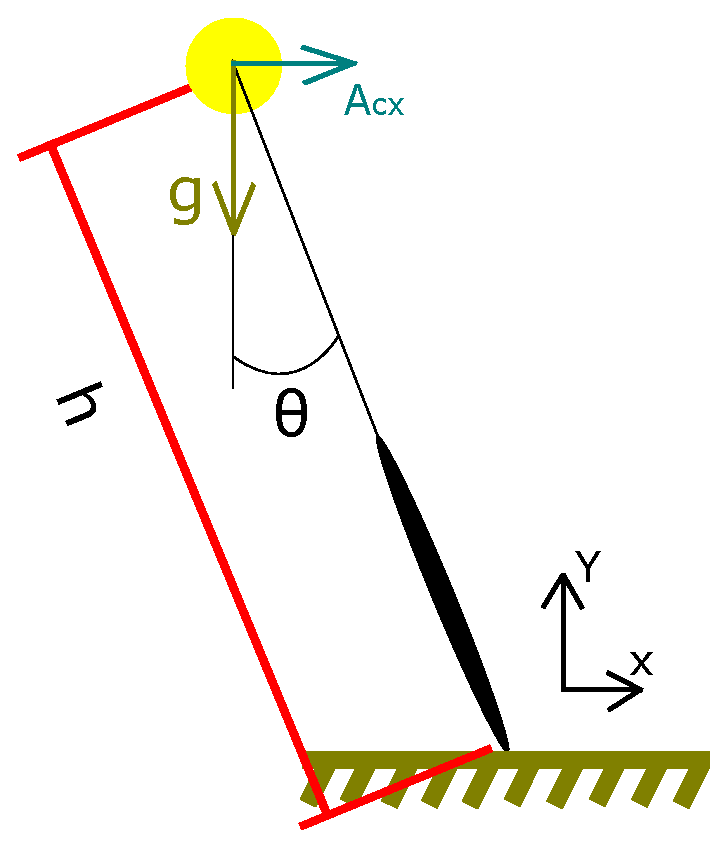
\includegraphics[width=4cm]{imagens/geometria/VistaTraseira.eps}
                \caption{Vista Traseira Esquemática}
            \end{figure}
            
            Até agora foi feita uma omissão de parâmetros. $\alpha$ e $\theta$ são funções do tempo, entretanto o parâmetro $(t)$ continuará sendo omitido a fim de tornar mais elegante as equações, ou seja, $\theta(t) = \theta$ e $\alpha(t) = \alpha$.

            A modelagem da Equação Diferencial será obtida através do método Newtoniano, através da somatória de momentos angulares:
            
            \begin{equation}
                J_z \ddot\theta = \sum M_z  = a_{cx}(\alpha) \cos(\theta)mh + \sin(\theta)gmh
            \end{equation}
            
            Sendo $J_z$ o momento de inercia em relação ao eixo $Z'$, e para $J_z=mh^2$ temos que:
            
            \begin{eqnarray}
                \ddot \theta =  \frac{a_{cx} (\alpha) \cos (\theta)  + \sin (\theta) g}{h}
            \end{eqnarray}
        
        \subsection{Validação do Modelo}
        
            A validação foi feita utilizando a equação diferencial sem qualquer linearização ou aproximação, para assim, considerar todas as dinâmicas da planta, para qualquer que sejam os valores de $\alpha$ e $\theta$. Para tal, foram utilizado dois métodos semelhantes, ambos em malha aberta.
            
            O primeiro consiste em partir da mesma condição inicial na equação diferencial e planta física, e zerar a entrada de ambas, o que desconsidera a dinâmica do atuador, ou seja, reduz a quantidade de variáveis que influenciam característica da resposta da saída para apenas $g$ e $h$. Como não convém alterar o valor de $g$, é então feito um ajuste fino em $h$ comparando o comportamento de ambas saídas.
            
            O segundo método consiste em também partir da mesma condição inicial, porém aplicando um degrau de mesma amplitude no mesmo instante de tempo na entrada de ambas, assim, considerando a dinâmica do atuador, o que faz surgir mais três variáveis que influenciam na característica de resposta da saída, sendo elas $d_{CG}$, $d$ e $v$, ou seja, são estas agora as variáveis a serem ajustadas comparando o comportamento de ambas saídas (já que  $g$ não convém ser alterada e $h$ já foi determinada pelo método anterior).
            
            Para aplicar ambos métodos foi utilizando o \textit{software MATLAB} para captar dados em tempo real da planta, e com o auxilio da extensão \textit{Simulink} para simular o modelo.foi utilizada a E.D. substituindo os valores inicialmente por obtidos através de medições da planta física. 
            
            Depois de sucessivos testes foi efetuada a validação da planta, esta pode ser resumida nos dois gráficos abaixo. 
            
            Este primeiro é a curva de validação zerando a entrada da planta, ou seja, desconsiderando a dinâmica do atuador: 
            
            \begin{figure}[h]
                %\centering
                \hspace{-15mm}
                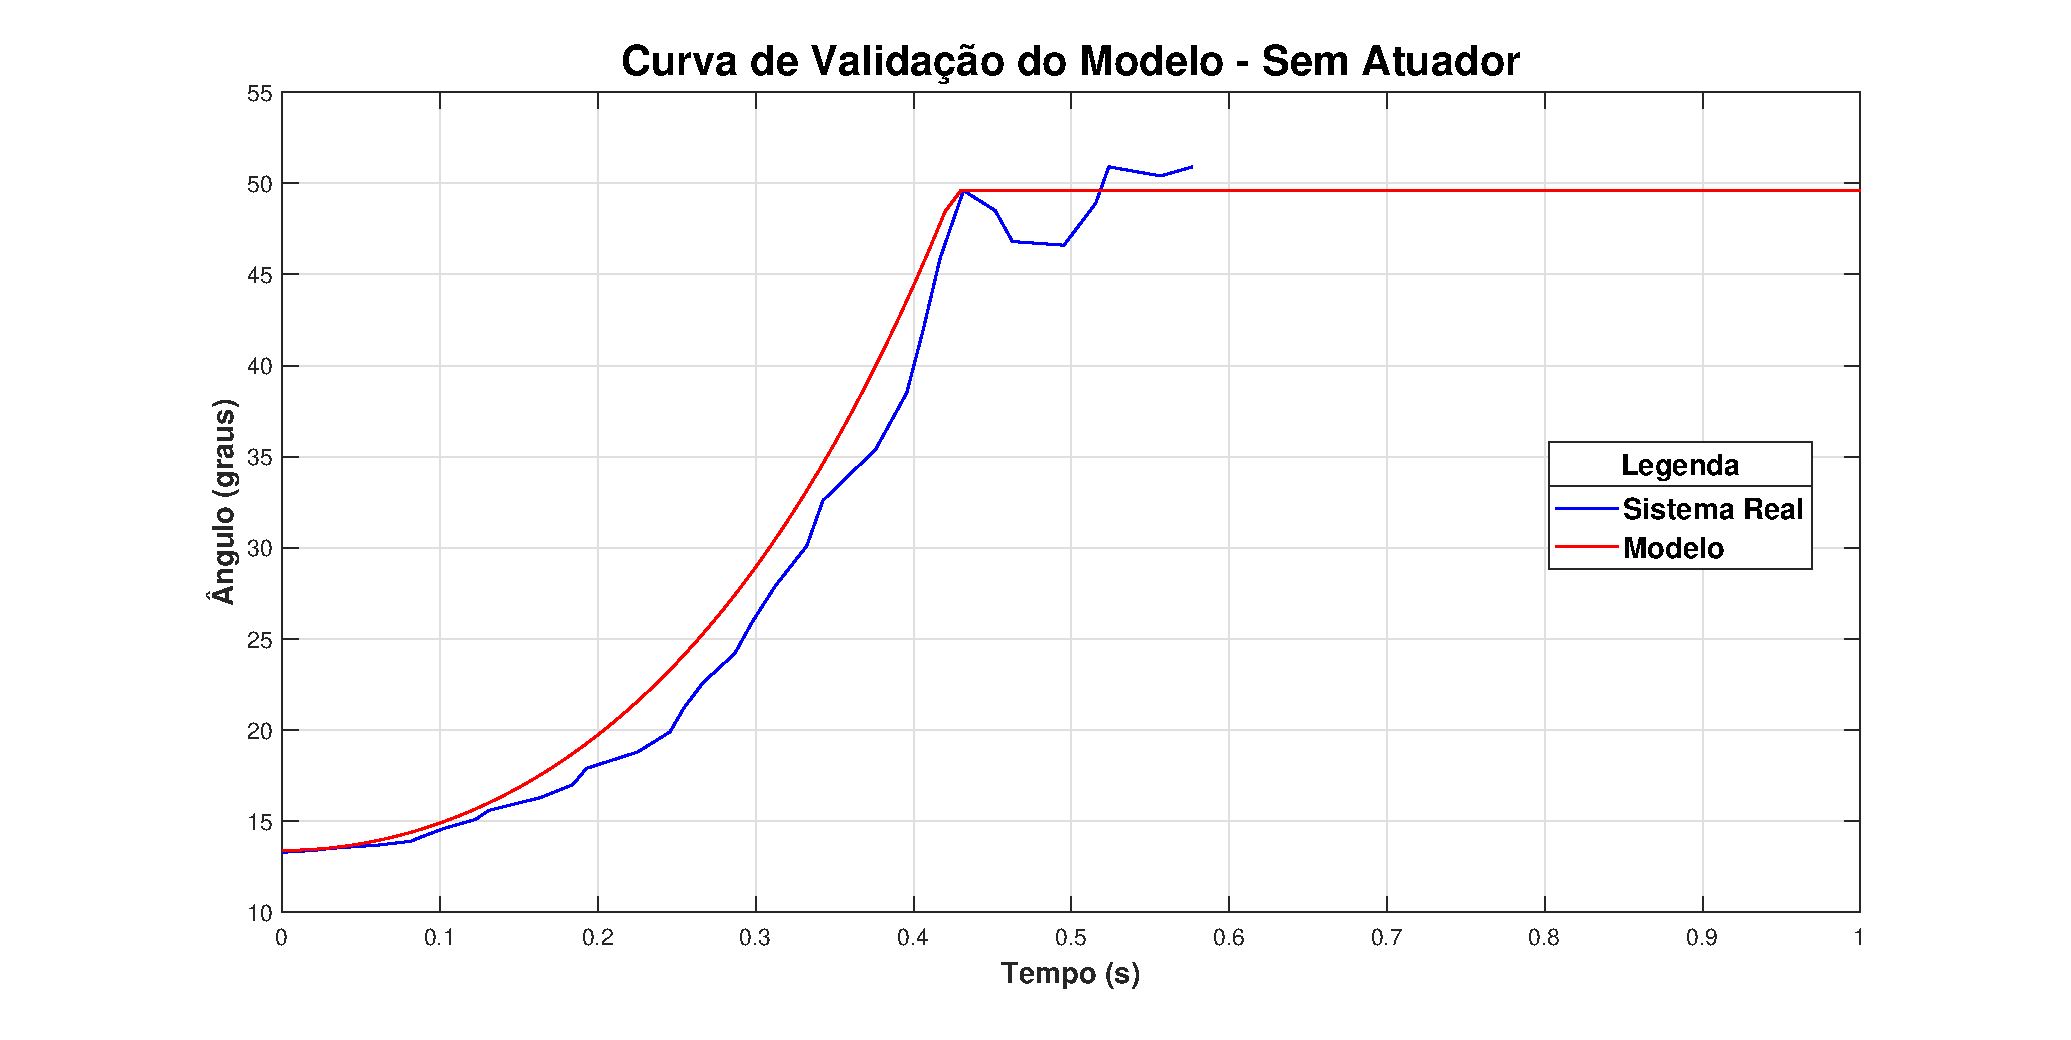
\includegraphics[width=10cm]{imagens/graficos/ValidacaoSemAtuador.eps}
                \caption{Validação Desconsiderando Dinâmica do Atuador}
            \end{figure}
            
            Este segundo consiste em aplicar um degral na entrada da planta de de $4º$ de amplitude instante $0s$ para duas condições iniciais diferentes, $\theta(0) = 13º$ e $\theta(0) = 16º$, ambas com $\dot\theta(0)=0rad/s$:
            
            \begin{figure}[H]
                %\centering
                \hspace{-15mm}
                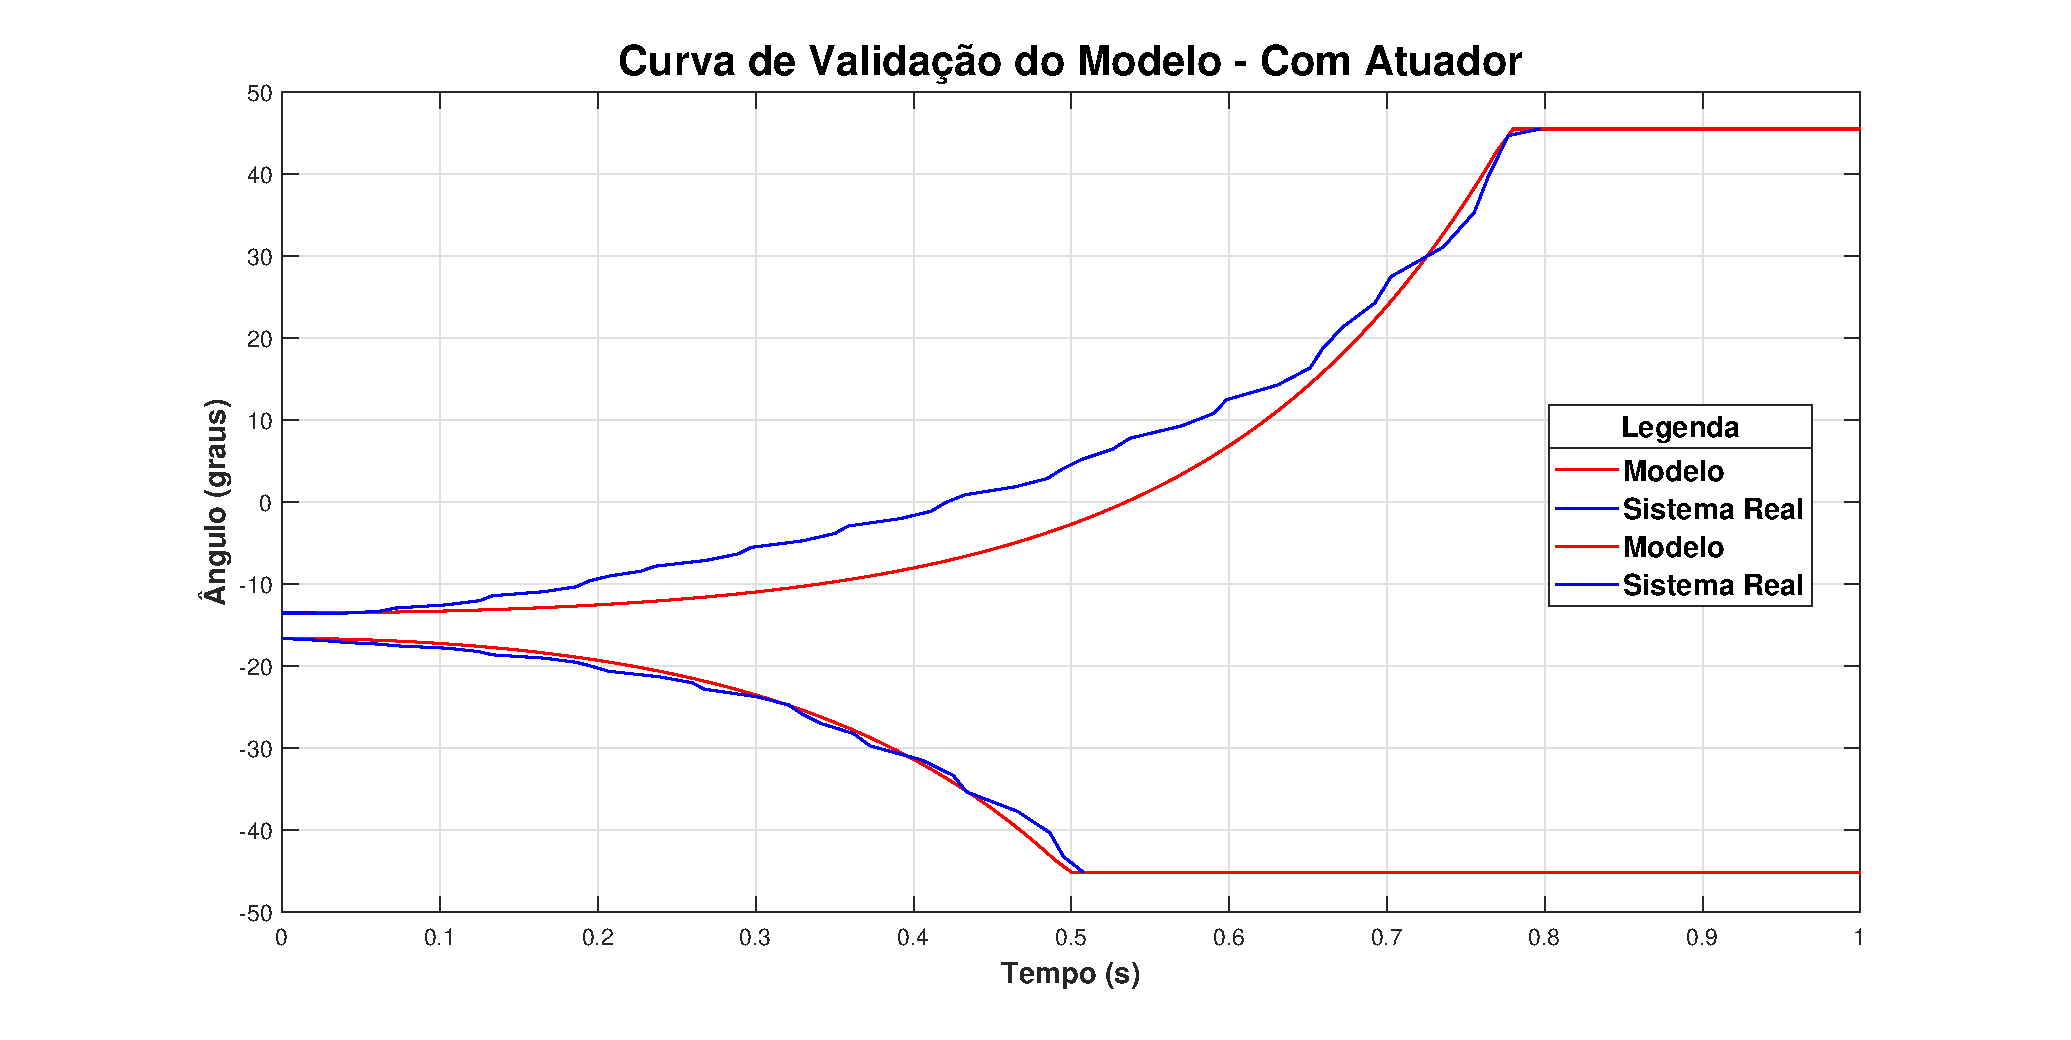
\includegraphics[width=10cm]{imagens/graficos/ValidacaoComAtuador.eps}
                \caption{Validação Considerando Dinâmica do Atuador}
            \end{figure}
            
            Por fim, os valores obtidos da validação são encontrado na seguinte matriz de equações:
            
            \begin{eqnarray}
                d_{CG} = 0,04m \nonumber\\
                d = 0,135m \nonumber\\
                h = 0,204m \nonumber\\
                v = 1,1  m/s \nonumber\\
                g = 9,807m/s^2
            \end{eqnarray}
        
        \subsection{Linearização do Modelo e Obtenção da Função de Transferência}
        
            Primeiramente é preciso definir um ponto de operação, O ponto de operação estabelecido para a entrada e a saida é $(\alpha,\theta)=(0,0)$. Assim sendo, linearizando $sen(\alpha)$ e $cos(\alpha)$ em torno de $\theta=0$ pela Serie de Taylor obtemos que $cos(\theta) \approx 1$ e $sen(\theta) \approx \theta$. Considerando ainda a linearização de $a{cx}$ obtida na subseção passada, é possível obter uma equação diferencial ordinária linearizada e aproximada para descrever o comportamento da planta, que esta é dada pela equação abaixo:
                
                \begin{equation}
                    \ddot\theta = \frac{a(\alpha) + g\theta}{h} = \frac{ \frac{v^2\alpha}{d} + g\theta}{h} =  \frac{v^2\alpha}{hd} + \frac{g\theta}{h}
                \end{equation}
                
            Explicitando $\alpha$ e $\theta$ que são funções do tempo, a fim de efetuar a troca de domínio, e tendo em vista que domínio $t$ (tempo) será levado no domínio $s$ (frequência) pela Transformada de Laplace, temos que:
            
            \begin{eqnarray}
                \mathcal{L} [\theta(t)] = \Theta(s)   \nonumber \\
                \mathcal{L} [\alpha(t)] = A(s)
            \end{eqnarray}
            
            Aplicando a Transformada de Laplace em ambos lado da E.D.O. linearizada temos:
            
            \begin{equation}
                 \mathcal{L} [\ddot\theta(t)] = \mathcal{L} [\frac{v^2\alpha(t)}{dh} + \frac{g\theta(t)}{h}]
            \end{equation}
            
            Como a Trasformada de Laplace é uma Transformadada Linear, obtemos o seguinte resultado:
            
            \begin{equation}
                s^2\Theta(s) - s\theta(t)|_0 - \dot\theta(t)|_0 = \frac{v^2A(s)}{dh} + \frac{g\Theta(s)}{h}
            \end{equation}
            
            As condições iniciais serão consideradas nulas, ou seja, $\theta(0) = 0$ e $\dot\theta(0)=0$, logo:
            
            \begin{eqnarray}
                \frac{v^2A(s)}{dh} = s^2\Theta(s) - \frac{g\Theta(s)}{h} \nonumber \\
                \Rightarrow    A(s) = s^2\Theta(s)\frac{hd}{v^2} - \Theta(s)\frac{gd}{v^2}
            \end{eqnarray}
            
            
            E então é obtido função de transferência arbitraria da planta:
            
            \begin{equation}
                G(s)= \frac{\Theta(s)}{A(s)} = \frac{1}{\frac{dh}{v^2}s^2 - \frac{gd}{v^2}} = (\frac{v^2}{d})\frac{1}{h {s^2} - g}
            \end{equation}
           
                Para obter a função de transferência da planta construída, basta substituir os valores obtidos na validação dados pela matriz de equações (13), onde temos que:
                
                \begin{equation}
                    G(s)= 8.963 \frac{1}{0.204s^2 - 9.807}
                \end{equation}
        
    \section{Projetos de Controladores}
    
        A palavra "sistema" será utilizada nesta seção em diante se referindo a um sistema de malha fechada que tem como componentes uma "planta" e um "controlador".
    
        \subsection{Controlador Proporcional - Método do Lugar Geométrico da Raízes}
        
            O Método do Lugar Geométrico da Raízes, LGR, visa analisar uma função de transferência de malha aberta de um sistema qualquer, a fim de determinar o comportamento dos seus polos de malha fechada a medida que é variada o ganho de realimentação do sistema de 0 a $\infty$. Para esboço do método é igualdo a $0$ a equação característica da função de transferência de malha fechada.
            
            O diagrama de blocos dado pela figura abaixo representa o sistema $T(s)$ para uma realimentação negativa de malha em $G(s)$ com ganho K arbitrário.
            
            \begin{figure}[h]
                %\hspace{-5mm}
                \centering
                \includegraphics[width=8cm]{imagens/graficos/DiagramaK.png}
                \caption{Diagrama de Blocos de $T(s)$}
            \end{figure}
            
            A função de transferência do sistema $T(s)$ é dada pela equação abaixo:
            
            \begin{equation}
                T(s) =  \frac{KG(s)}{1+KG(s)}
            \end{equation}
            
            O LGR pode ser esboçado com o auxilio da função $rlocus()$ do \textit{software MATLAB}. A figura abaixo é o esboço do LGR de $1+KG(s)=0$.
            
            \begin{figure}[h]
                %\centering
                \hspace{-10mm}
                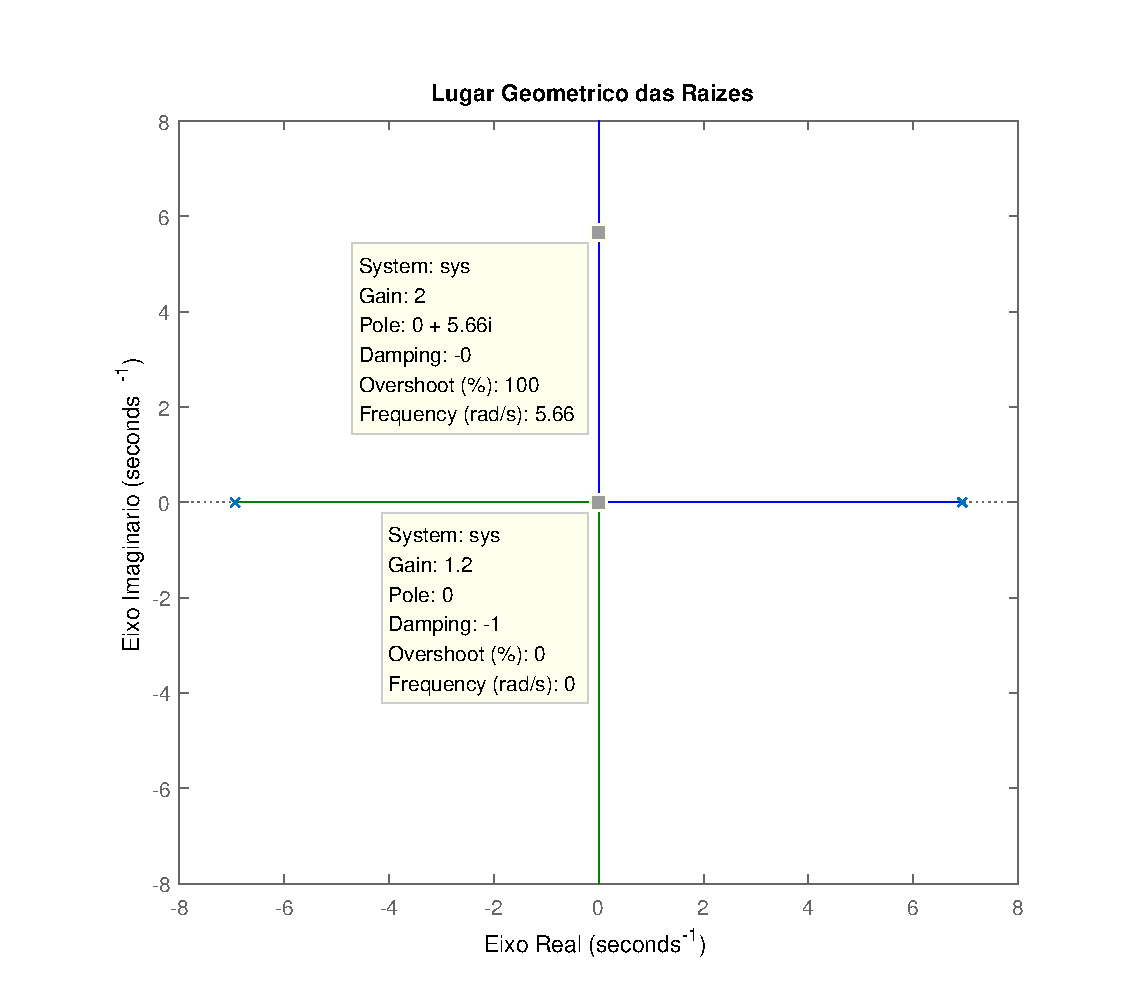
\includegraphics[width=9cm]{imagens/graficos/LGR-Kp.eps}
                \caption{LGR de $1+KG(s)$}
            \end{figure}
            
            Analisando o LGR de $1+KG(s)$ chegamos a conclusão que $T(s)$ é instável, ou seja, possui polos no semi-plano direito, para $0\leq K < 1.2$, e $T(s)$ é marginalmente estável para $K\geq1.2$. Em outras palavras não exite um ganho K que torne $T(s)$ assintoticamente estável.
           
            Afim de testes foi projetado ganho $K=1.5$ que torna o sistema marginalmente estável, com polos localizados em $+/-1.2j$.
            
            \subsection{Controlador Proporcional e Derivativo}
            
            Será feita uma tentativa de projetar um controlador Proporcional e Derivativo, PD, usando novamente o LGR e o aproveitando o ganho projetado na subseção anterior.
            
            O controlador tem função de transferência $C(s) = K_p + sK_d$ e o diagrama de blocos do novo sistema, $F(s)$, pode ser visto na figura abaixo:
            
            \begin{figure}[h]
                \centering
                %\hspace{-5mm}
                \includegraphics[width=8cm]{imagens/graficos/DiagramaKD.png}
                \caption{LGR de $1+K_dG(s)$}
            \end{figure}
            
            A função de transferência do novo sistema é dada por $F(s) = \frac{C(s)G(s)}{1+C(s)G(s)}$ e o LGR pode é obtido pela equação característica $1+C(s)G(s)=0$. Re-proveitando o ganho projetado na subseção anterior temos que $K=K_p=1.5$, logo:
            
            \begin{equation}
                0 = 1 + C(s)G(s) = 1 + 8.963\frac{1.5 + sK_d}{0.204s^2 - 9.807}
            \end{equation}
            
            Onde é possível reorganizar esta equação de forma a isolar $K_d$ e obter:
            
            \begin{equation}
                0 = 1 + K_d\frac{8.963s}{0.204s^2 + 3.6375} = 1 + K_dQ(s)
            \end{equation}
            
            Já no formato adequado para aplicar o método do LGR é possível utilizar a ferramenta $rlocus()$, onde o resultado pode ser visto na figura abaixo:
            
            \begin{figure}[h]
                %\centering
                \hspace{-18mm}
                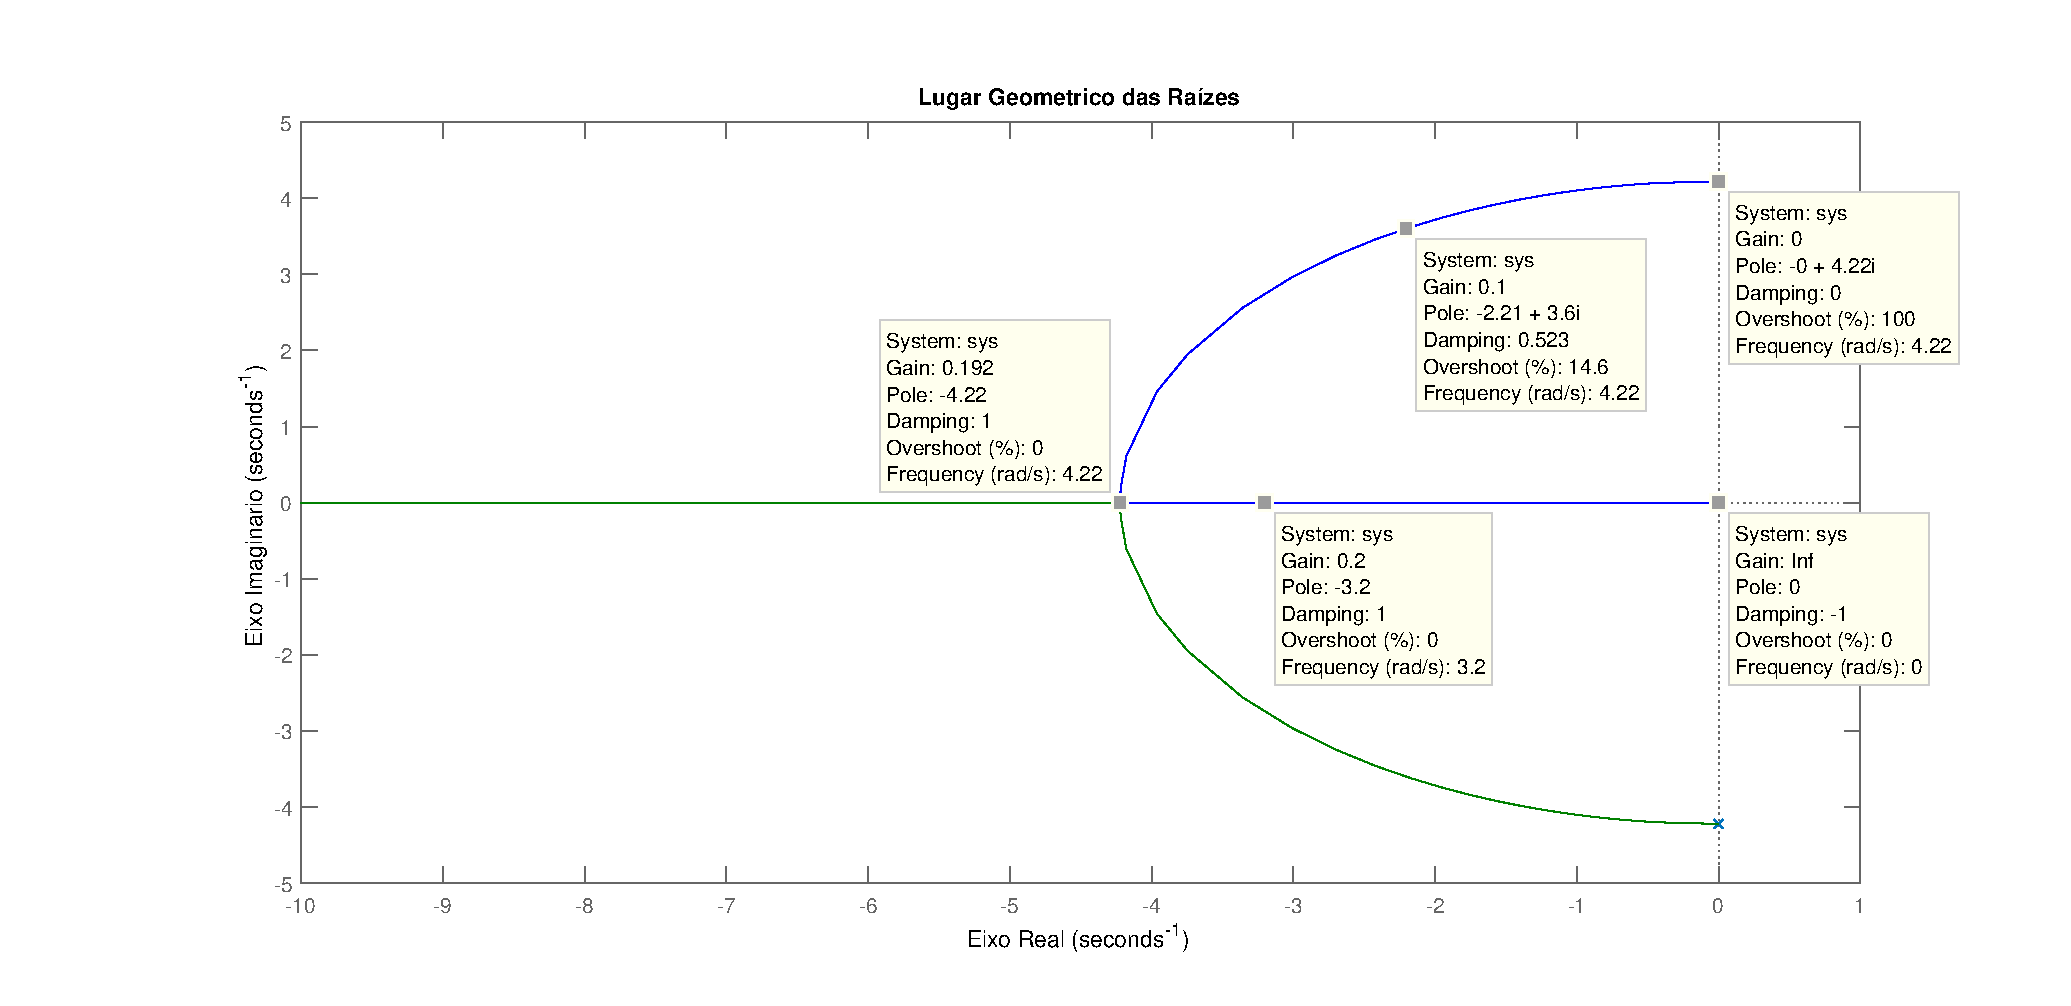
\includegraphics[width=10cm]{imagens/graficos/LGR-Kd.eps}
                \caption{LGR de $1 + K_dQ(s)$}
            \end{figure}
            
            Analisando o LGR concluímos que para $K_d=0$ o sistema é marginalmente estável, como esperado, para $0 < K_d < 0.192$ o sistema é estável com polos complexos conjugados, e para $ K_d \geq 0.192$ o sistema é estável com polos no eixo real.
            
            Caso desejado obter um \textit{overshoot} de aproximadamente $14.6$, por exemplo a fim de testes, basta fazer $K_d = 0.1$.
            
            O sistema resultante, $F(s)$, tem função de transferência arredondada pela equação abaixo:
            
            \begin{equation}
                F(s) \approx 4.39 \frac{(15+s)}
                {(s^2 + 4.39s + 17.83)}
            \end{equation}
            
            Os polos e zeros da equação exata de $F(s)$ podem ser observados graficamente pela figura abaixo, obtida pela função $pzmap()$ também do \textit{software MATLAB}.
            
            \begin{figure}[h]
                %\centering
                \hspace{-18mm}
                \includegraphics[width=10cm]{imagens/graficos/pzmap.eps}
                \caption{Mapa de polos e zeros de $F(s)$}
            \end{figure}
            
            Em suma, foi projetado um controlador não causal, $C(s) = 1.5 + s0.1$, que torna o sistema em malha fechada estável. O sistema resultante possui com polos complexos conjugados em $-2.21 \mp3.6i$, que estes resultam em um fator de amortecimento igual a $0.523$, máximo overshoot percentual de $14.6$ e frequência natural igual a $4.22rad/s$.
        
    \section{Resultados e Discussões}
    
        \subsection{Testes com o Controlador Proporcional}
            
            Esta experiencia foi realizada na planta alterando inicialmente os parâmetros do controlador PID embarcado para o equivalentes ao projeto da subseção 6.1, que seriam $K_p=1.5$, $K_d=0$ e $K_i=0$, com a maior taxa de amostragem que o sensor e microcontrolador suportarem a fim de simular o domínio continuo.
            
            A simulação da mesma foi feita com o auxilio do \textit{softwere MATLAB Simulink}, para o sistema de malha fechada da figura 7 com o valor de $K=1.5$.
            
            Os resultados da experiencia e da respectiva simulação podem ser comparados no gráfico abaixo:
            
            \begin{figure}[h]
                %\centering
                \hspace{-15mm}
                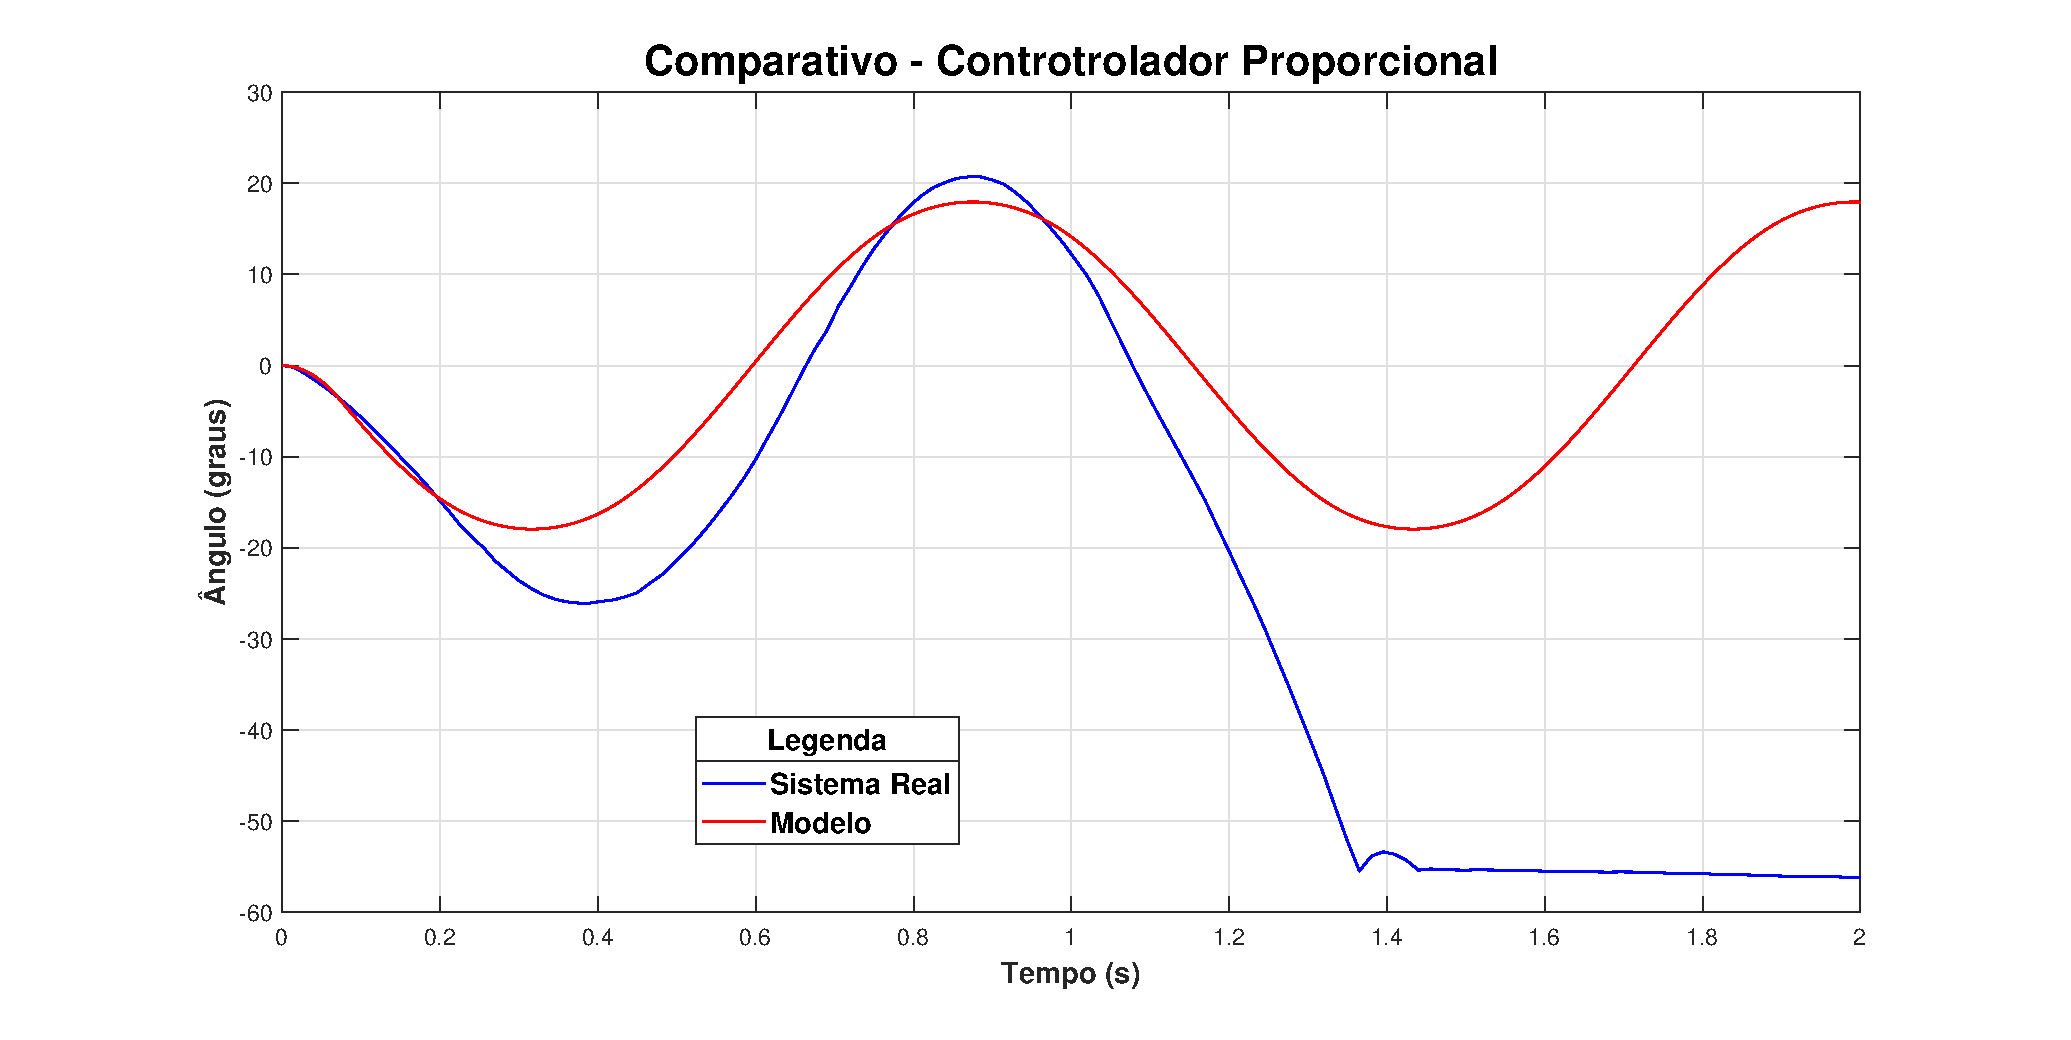
\includegraphics[width=10cm]{imagens/graficos/ComparativoP.eps}
                \caption{Resultado dos testes com controlador Proporcional}
            \end{figure}
            
            Na simulação do sistema $T(s)$, planta com o controlador proporcional, a característica de resposta é marginalmente estável, em contra-partida, no experimento do mesmo ele obteve uma característica de resposta instável.
            
        \subsection{Testes com o Controlador Proporcional e Derivativo}
            
            Esta experiencia foi realizada na planta alterando os parâmetros do controlador PID embarcado para o equivalentes ao projeto da subseção 6.2, que seriam $K_p=1.5$, $K_d=0.1$ e $K_i=0$, também com a maior taxa de amostragem possível.
            
            A simulação da mesma também foi feita com o auxilio do \textit{softwere MATLAB Simulink}, para o sistema de malha fechada da figura 8 com os valores de $K_p=1.5$ e $K_d=1.5$.
             
            Os resultados desta experiencia e sua respectiva simulação podem ser comparados no gráfico abaixo:
            
            \begin{figure}[h]
                %\centering
                \hspace{-18mm}
                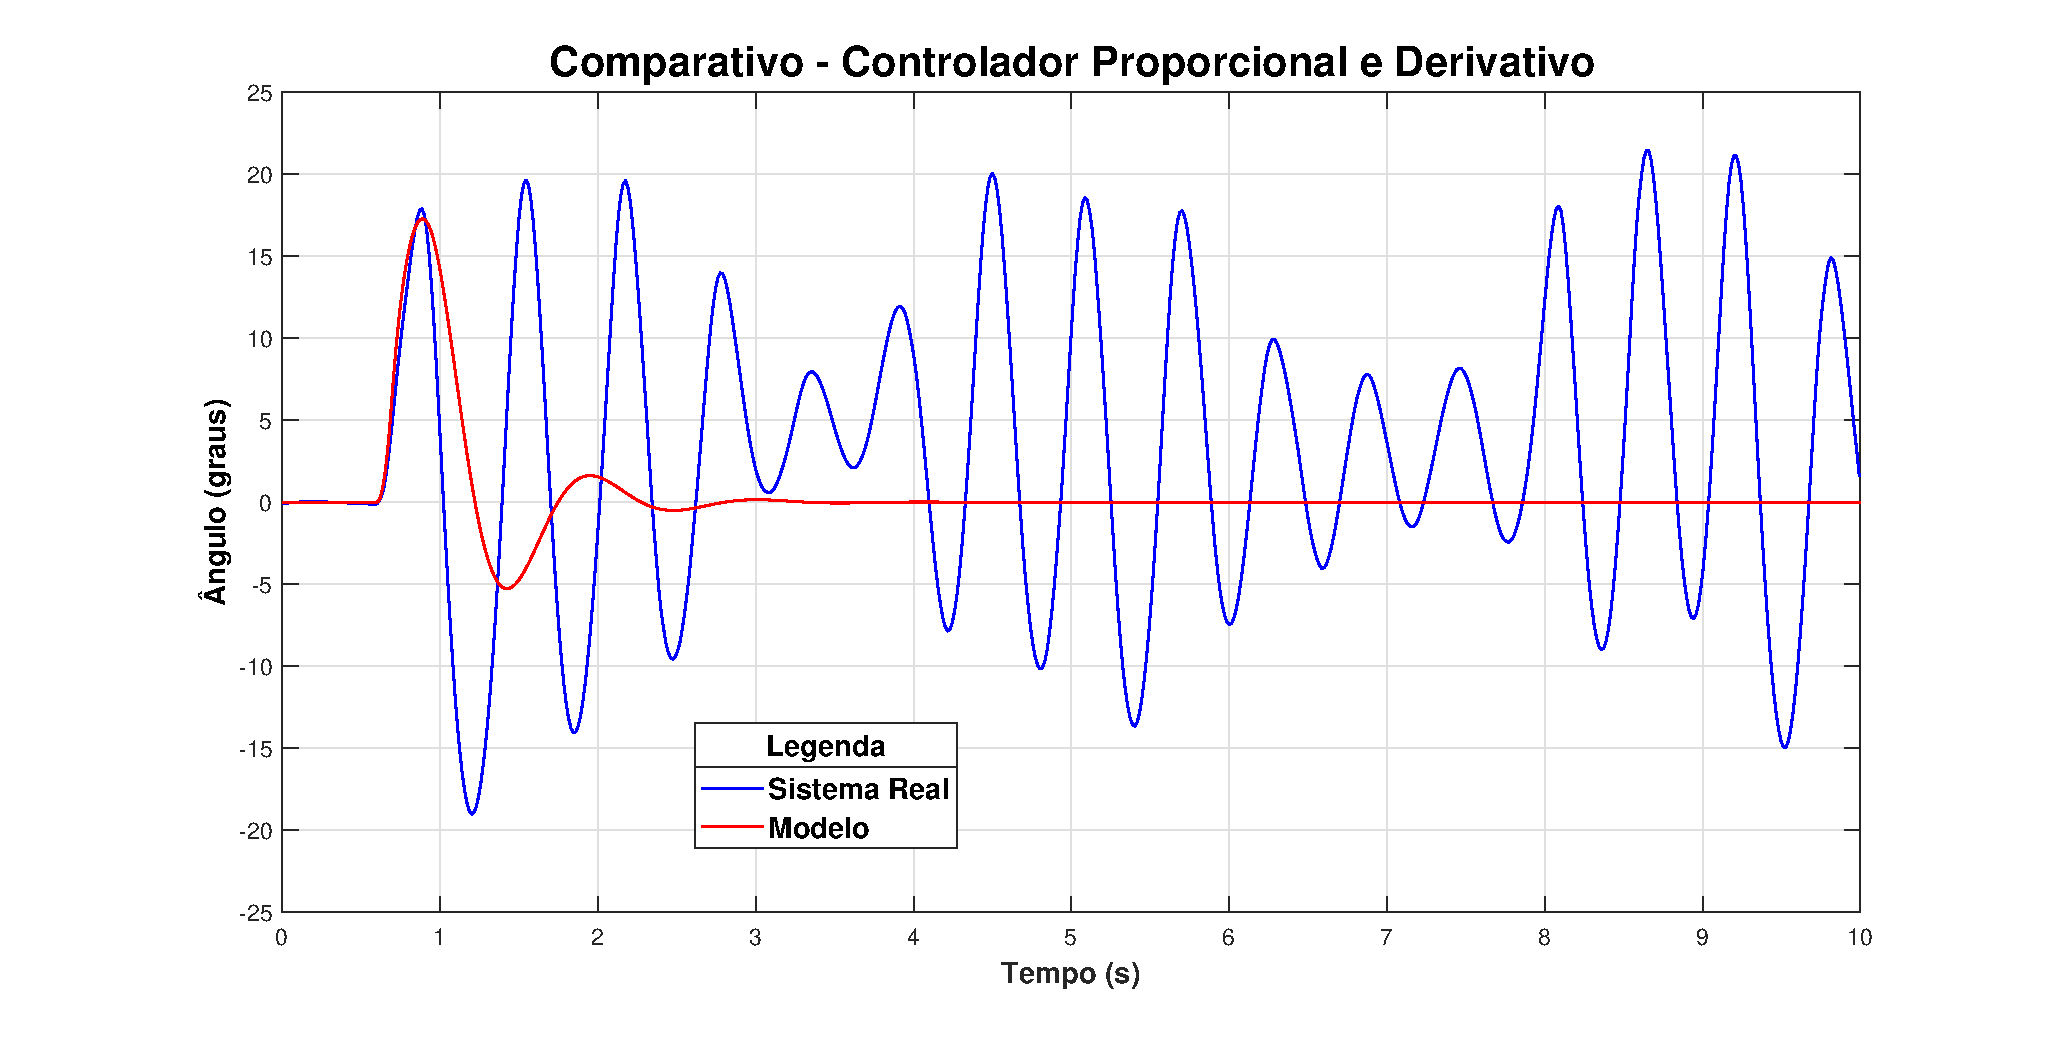
\includegraphics[width=10cm]{imagens/graficos/ComparativoPD.eps}
                \caption{Resultado dos testes com controlador Proporcional e Derivativo}
            \end{figure}
            
            Já na simulação do sistema $F(s)$, planta com o controlador proporcional e derivativo, a característica de resposta é assintoticamente estável, em contra-partida, no experimento do mesmo ele obteve uma característica de resposta oscilante.
            
        \subsection{Discussões}
            
            Naturalmente os resultados das experiencias e simulações são bem diferentes. Isso se deve a vários possíveis motivos, dentre os principais: Linearizações e aproximações, já que os sinais fogem do ponto de operação. Influencias de pertubações externas imprevisíveis. Possíveis desconsiderações e erros de modelagem. E desconsideração da dinâmica do atuador, já que a dinâmica do mesmo é desconhecida, e então foi partido do pressuposto que a mesma seria $1$. Inconstância na velocidade, já que o atuador que controlaria a mesma é operado até então em malha aberta e os ganhos do controlador não são realimentados com a mesma.
        
    \section{Considerações Finais e Propostas Futuras}
            
            A metodologia de partir do modelo de Equação Diferencial para obter a função de transferência da planta para obter informações como por exemplo característica de resposta em malha aberta de demostrou-se útil.
            
            O método do LGR demonstrou-se um método eficaz de prever o comportamento do sistema em malha fechada e para projetar de controladores.
            
            O controlador proporcional e derivativo demonstrou-se mais eficaz em relação a apenas o controlador proporcional, devido a vantagem do mesmo ter a capacidade de deslocar os para o lado esquerdo do eixo $j\omega$.
            
            Ficam como propostas futuras: Rever o modelo da planta procurando possíveis erros de modelagem e revendo desconsiderações feitas. Considerar a dinâmica do atuador, para isso, descobrir a dinâmica do atual atuador ou troca-lo.  Realimentar a velocidade tangencial para projetar um controlador para a mesma, além disso, projetar um controlador mais eficaz para o controle de inclinação levando em conta a velocidade tangencial. E por fim, fazer uso de outras técnicas de controle mais avançadas.
    
    \section{Revisão Bibliográfica}
    
        Murray, R. M. and Aström, K. J. (2009), Feedback control systems, 2th ed., Princeton University Press, Woodstock, Oxfordshire.
        
        Dorf, R. C and Bishop, R. H (2008), Modern Control Systems, 11th ed., Prentice-Hall, California, CA.
        
        OGATA, Katsuhiko. Engenharia de controle moderno. 3. ed. Rio de Janeiro: Prentice Hall, c1998.
        
\end{document}